\chapter{Realization}
\label{ch:setup}

\section{Simulation model creation}

\subsection{Microsoft Project plugin}

\subsection{Unity plugin}

\subsection{Unity simulation creation}

The simulation is also faster than recording the data. We can generate a lot of data in a short time. The simulation is also cheaper than recording the data. We don't need to buy a vehicle and a camera to generate the data. We only need to buy a microphone and a speaker. The simulation is also more flexible than recording the data. We can change the position of the microphone and the camera easily. We can also change the vehicle's speed and the number of vehicles in the simulation. The simulation is also more reproducible than recording the data. We can generate the same data multiple times. We can also generate data for the same position of the sound source multiple times. The simulation is also more scalable than recording the data. We can generate data for any position of the sound source. We can also generate data for any number of vehicles. The simulation is also more controllable than recording the data. We can control the position of the sound source, the vehicle's speed, and the number of vehicles. The simulation is also more secure than recording the data. We can generate data without any risk of accidents. The simulation is also more accessible than recording the data. We can generate data without

\section{Dataset creation}

\subsection{Microphone installation}

To record real data that suits our baseline, we must design a system to record and save lots of data. As we had the opportunity to place it on the HEIA-FR, we decided to design a system containing an embedded system, two microphones, a camera, and an embedded system. For the hardware, we chose to ensure that the system is easily replicable and that the system is not too expensive. We used hardware available at the HEIA and at Rosas. The system design is shown in Figure \ref{fig:real_data_recording_system}.

\begin{figure}[H]
    \centering
    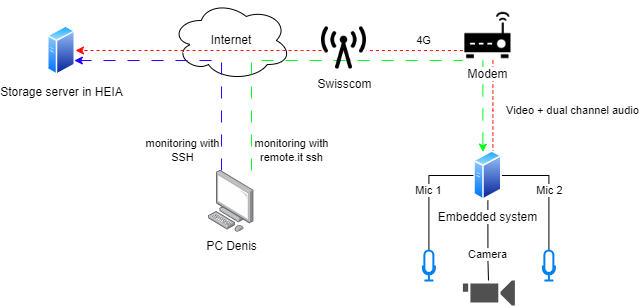
\includegraphics[width=1\textwidth]{../Images/real_data_recording_system.drawio.png}
    \caption{Real data recording system}
    \label{fig:real_data_recording_system}
\end{figure}

Red flow, green flow, blue flow

\subsection{Embedded system setup and access}

The setup can be easily replicated in many other environments, such as other city streets, traffic intersections, etc. This setup is a valuable starting point to develop and test a system that can accurately identify and track sound sources.

\subsection{Data transmission}

\subsection{Data recording and storage}

\section{Neural Network for Sound Source Localization}

\subsection{Dataset preparation}

\subsection{Neural Network architecture}

\subsection{Training}

\section{Adversarial Attack}

\subsection{Fast Gradient Signed Method implementation}

